\chapter{Registrierung}
\label{cha:register}

Die Registrierung ist auf der Startseite links unten (Abbildung  \ref{fig:view_login} \textit{\nameref{fig:view_login}}) zu finden.

\vspace*{5mm} \noindent Alle Felder sind Pflichtangaben. Wenn die selbe E-Mail Adresse wie beim eigenen Facebook Account verwendet wird, ist später ein Facebook Direkt-Login möglich. Das Passwort wird in der Datenbank verschlüsselt abgelegt. Es kann nicht vom Administrator gelesen werden.

\begin{figure}[h]
 \begin{addmargin}{-0.2\linewidth}
   \centering 
   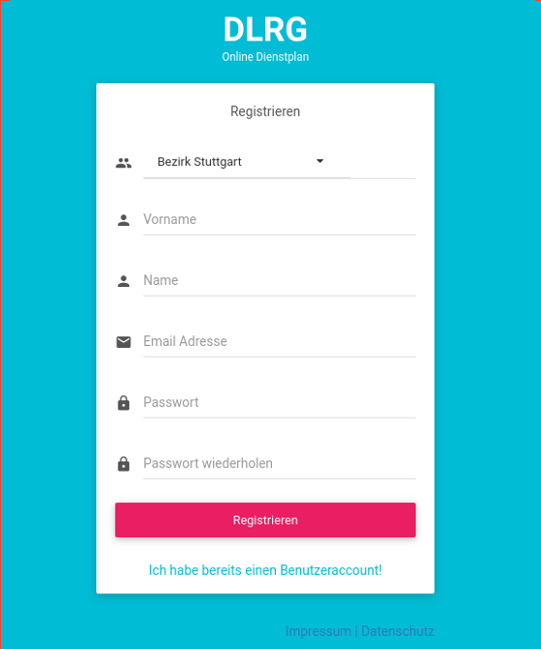
\includegraphics[width=10cm]{Bilder/view_register.png}
 \end{addmargin} 
 \caption[Registrierungs ansicht]{DLRG Dienstplan Registrierungs ansicht}
 \label{fig:view_register}
\end{figure}

\vspace*{5mm} \noindent 
Nachdem auf Registrieren geklickt wurde, muss der Account von einem Administrator freigeschaltet werden. Der Benutzer wird mit einer automatischen E-Mail benachrichtigt. 

\noindent Nach dem Login kann optional im Profil (siehe Kapitel \ref{sec:menu_profile} \textit{\nameref{sec:menu_profile}}) noch die Handynummer hinterlegt werden.